%----------------------------------------------------------------------------------------
%	PACKAGES AND THEMES
%----------------------------------------------------------------------------------------
\documentclass[aspectratio=169,xcolor=dvipsnames]{beamer}
\usetheme{SimplePlus}

\usepackage{hyperref}
\usepackage{graphicx} % Allows including images
\usepackage{booktabs} % Allows the use of \toprule, \midrule and \bottomrule in tables
\usepackage{siunitx}
\usepackage{import}
\usepackage{amsmath}
%\numberwithin{equation}{section}% numera eq come #section.#formula
\usepackage{amsthm}
\usepackage{stmaryrd}
\usepackage{amssymb}
\usepackage{wasysym}
\usepackage{cancel}
\usepackage{textcomp}
\definecolor{myred}{rgb}{0.545, 0.172, 0.031}
%\usepackage{cleveref}
%----------------------------------------------------------------------------------------
%	TITLE PAGE
%----------------------------------------------------------------------------------------

\title[short title]{Omogeneizzazione numerica di materiali microstrutturati} % The short title appears at the bottom of every slide, the full title is only on the title page
\subtitle{Omogenizzazione di tessuto osseo}

\author[Pin-Yen] {Alessandro Mastrofini}

\institute[NTU] % Your institution as it will appear on the bottom of every slide, may be shorthand to save space
{
Meccanica Computazionale dei Tessuti e Biomateriali \\
Università degli Studi di Roma Tor Vergata% Your institution for the title page
}
\date{2022} % Date, can be changed to a custom date

\graphicspath{{figures/}} %Setting the graphicspat%h
\graphicspath{{figures/}} %Setting the graphicspath
\makeatletter
\providecommand*{\input@path}{}
\edef\input@path{{figures/}{}\input@path}% prepend
\makeatother
%----------------------------------------------------------------------------------------
%	PRESENTATION SLIDES
%----------------------------------------------------------------------------------------

\begin{document}

\begin{frame}
    % Print the title page as the first slide
    \titlepage
\end{frame}

%------------------------------------------------
\section{First Section}
%------------------------------------------------

\begin{frame}{Volume di interesse}
    \begin{figure}%[b!]  %% Add a [b!] if you prefer the wide image to be at the bottm of the page
  	\centering
  	\tiny{\def\svgwidth{\textwidth}
  	\input{homogen2.pdf_tex}}
  \end{figure}

\end{frame}

\begin{frame}{Omogenizzazione}
	\begin{figure}
		\centering
		\begin{minipage}{0.45\linewidth}
			\begin{center}
	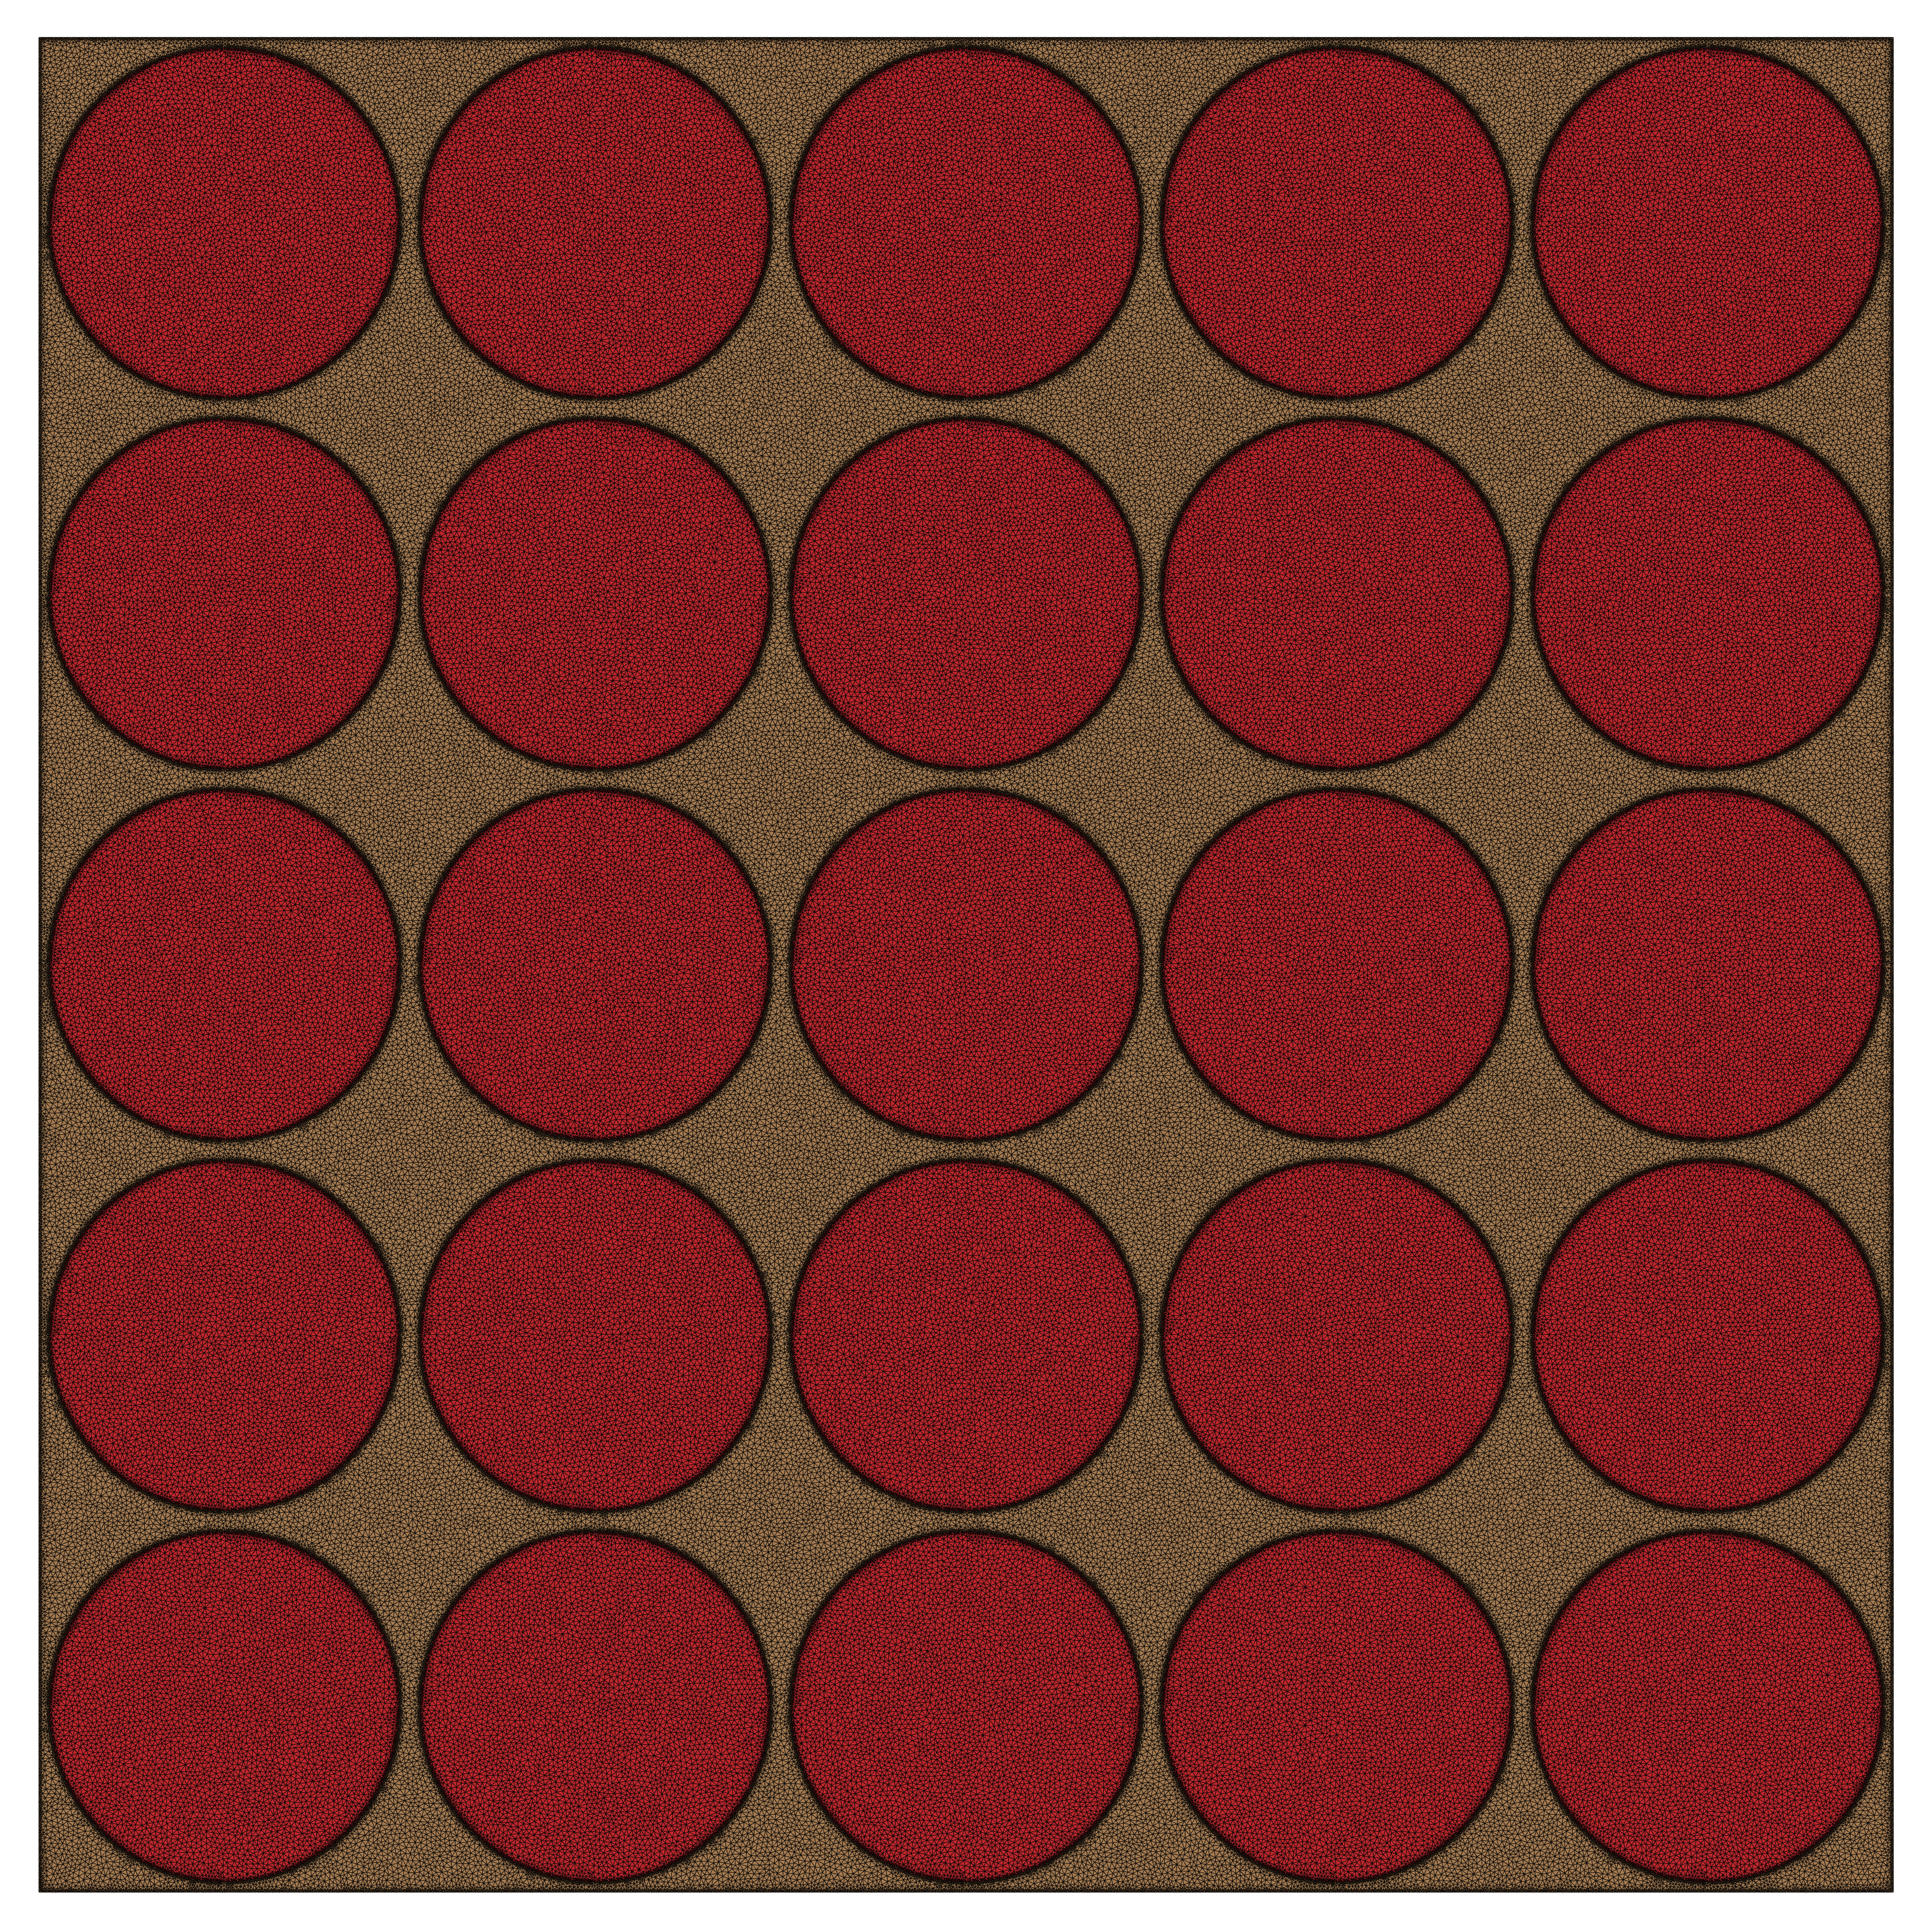
\includegraphics[width=0.5\linewidth]{test_mesh_8.png}
	\vspace{20pt}\vfill
	\small{$\mathbb{C}^{(o m)}=\left(\begin{array}{ccc}756.78 & 80.90 & 0.00 \\ 80.90 & 756.78 & 0.00 \\ 0.00 & 0.00 & 40.87\end{array}\right)$}
\end{center}
		\end{minipage}\hfill
		\begin{minipage}{0.51\linewidth}
		\tiny{	\def\svgwidth{\linewidth}
			\input{test_data1.pdf_tex}}
		\end{minipage}\hfill
	\end{figure}
\end{frame}
%------------------------------------------------

\begin{frame}{Microstruttura}
\begin{figure} 
	\centering
	\begin{minipage}[b]{0.16\linewidth}
		\centering
	\tiny	$\operatorname{AxR}=0.8	$
	\end{minipage}
	\begin{minipage}[b]{0.16\linewidth}
		\centering
	\tiny	$\operatorname{AxR}=0.6	$
	\end{minipage}
	\begin{minipage}[b]{0.16\linewidth}
		\centering
	\tiny	$	\operatorname{AxR}=0.5$
	\end{minipage}
	\begin{minipage}[b]{0.16\linewidth}
		\centering
	\tiny	$	\operatorname{AxR}=0.3$
	\end{minipage}
	\begin{minipage}[b]{0.16\linewidth}
		\centering
	\tiny	$	\operatorname{AxR}=0.1$
	\end{minipage} 
	\begin{minipage}[b]{0.16\linewidth}
		\includegraphics[width=\linewidth]{test_mesh_axR_0.8.png}
	\end{minipage} 
	\begin{minipage}[b]{0.16\linewidth}
		\includegraphics[width=\linewidth]{test_mesh_axR_0.6.png}
	\end{minipage} 
	\begin{minipage}[b]{0.16\linewidth}
		\includegraphics[width=\linewidth]{test_mesh_axR_0.5.png}
	\end{minipage}
	\begin{minipage}[b]{0.16\linewidth}
		\includegraphics[width=\linewidth]{test_mesh_axR_0.3.png}
	\end{minipage} 
	\begin{minipage}[b]{0.16\linewidth}
		\includegraphics[width=\linewidth]{test_mesh_axR_0.1.png}
	\end{minipage} 
\end{figure}

\begin{figure}[bt!] %% preferably at bottom or top of column
	
	\centering
	\tiny{	\def\svgwidth{0.40\linewidth}
\input{var_geometr.pdf_tex}}
\end{figure}

\end{frame}

%------------------------------------------------

\begin{frame}{Regione di interesse}
\begin{figure} 

	\begin{minipage}[c]{0.20\linewidth}
	\includegraphics[width=\linewidth]{mesh_100.png}
\end{minipage} \hspace{0.01\linewidth}
\begin{minipage}[c]{0.20\linewidth}
	\includegraphics[width=\linewidth]{mesh_300.png}
\end{minipage}\hspace{0.01\linewidth}
		\begin{minipage}[c]{0.20\linewidth}
			\includegraphics[width=\linewidth]{real_mesh_n1.png}
		\end{minipage}\hspace{0.01\linewidth}
		\begin{minipage}[c]{0.20\linewidth}
			\includegraphics[width=\linewidth]{real_mesh_n2.png}
		\end{minipage}
	
\end{figure}
\begin{figure}
				\centering
		\begin{minipage}[b]{0.22\linewidth}
			\tiny{$
				\begin{bmatrix}
					1034.17 & 411.96 & -11.69 \\
					411.96 & 1074.45 & -21.40 \\
					-11.67 & -21.41 & 224.12 \\
				\end{bmatrix}
				$}
		\end{minipage}\hspace{0.01\linewidth}
		\begin{minipage}[b]{0.22\linewidth}
			\centering
			\tiny{$
				\begin{bmatrix}
					959.28 & 439.22 & 0.29 \\
					439.21 & 995.56 & -11.64 \\
					0.29 & -11.63 & 209.55 \\
				\end{bmatrix}
				$}
		\end{minipage}\hspace{0.01\linewidth}
		\begin{minipage}[b]{0.22\linewidth}
			\centering
			\tiny{$
				\begin{bmatrix}
					1744.59 & 701.46 & 81.03 \\
					701.46 & 1649.60 & 49.05 \\
					81.03 & 49.05 & 540.63 \\
				\end{bmatrix}
				$}
		\end{minipage}\hspace{0.01\linewidth}
		\begin{minipage}[b]{0.22\linewidth}
			\centering
			\tiny{$
				\begin{bmatrix}
					2237.42 & 887.87 & 19.48 \\
					887.87 & 2394.87 & 71.54 \\
					19.48 & 71.54 & 690.04 \\
				\end{bmatrix}
				$}
		\end{minipage}		

\end{figure}

\end{frame}

\begin{frame}{Parametri materiali}
\begin{figure}
	\centering
	\begin{minipage}{0.45\linewidth}
	\tiny{\def\svgwidth{0.9\linewidth}
	\input{variazione_Ebone.pdf_tex}}
	\end{minipage}\hfill
	\begin{minipage}{0.51\linewidth}
	\tiny{\def\svgwidth{\linewidth}
\input{variazione_Enarrow.pdf_tex}}
\end{minipage}\hfill
\end{figure}
\end{frame}

\end{document}